\section{Разработка собственного програмного обеспечения для учета семейного бюджета}

Как правило систематическое занесение доходов и расходов в таблицу, а
также подсчет итогового баланса может оказаться весьма непростым занятием, но и использование электронных таблиц и специализированных программ
тоже не тривиальная задача, поскольку такие методы разрабатываются с учетом максимально широких возможностей использования, от самых простых
табличных расчетов и до учета дивидендов от приобретенных акций, что не
очень хорошо ложится на базовый семейный бюджет.

\subsection{Выбор языка программирования}

Поэтому я и решился на разработку своего приложения, которое будет
максимально комфортным в использовании и обладать набором функций,
которые необходимы мне,не очень сильно использовать ресурсы компьютера.
При выборе языка программирования для создания приложения я остановился на трех базовых концепциях:

\begin{enumerate}
\item Портируемость
\item Легкость
\item Удобство использования
\item Большие возможности
\end{enumerate}

Благодаря этому списку мне удалось достаточно сильно сократить число
языков программирования на которых можно было написать приложение, в
итоге я остановился на языке

C++ с расширением QT Framework. Который оказался достаточно комфортным и легко расширяемым для выполнения необходимых задач.

\subsection{Разработка базовой концепции приложения}
В качестве базовой концепции приложения был выбран вариант модифицированных электронных таблиц. Самым простым вариантом была следующая структура
\begin{enumerate}
\item Размер операции
\item "Сторона"операции (приход/расход)
\item Коментарий к операции
\item Дата и время операции
\end{enumerate}

Остаток вычислялся путем последовательного суммирования (с модификатором "стороны") размеров операции отсортированных по датам и времени
операции

\subsubsection{Начало разработки}
Первоначальная версия сущестовала в консольном виде без взаимодействия с курсором мыши. Данные хранились в текстовом виде, что позволяло
легко модифицировать записанные данные. Позже были добавлены категории записей, которые позволили однозначно делать подсчет расходов по категориям расходов.

\subsection{Разработка графической версии}
Немного позже был разработан первоначальный вариант графической версии приложения, он по прежнему записывал данные в файл и при этом работал достаточно неэффективно.

\begin{figure}[H]
	\centering
	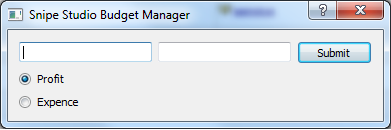
\includegraphics[width=0.7\linewidth]{pics/firstVersion.png}
	\caption{Первоначальный вариант графического приложения Budget Manager}
	\label{fig:firstVersion}
\end{figure}

Немного позднее было добавлено поле отображающее список операций

\begin{figure}[H]
	\centering
	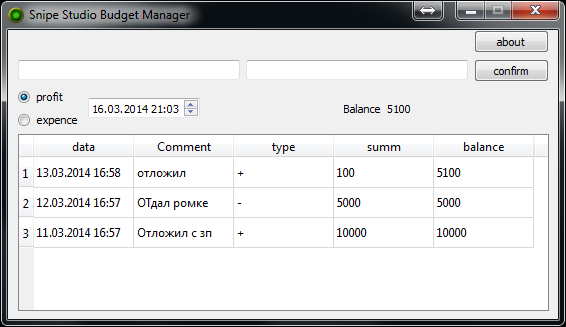
\includegraphics[width=0.7\linewidth]{pics/secondVersion.png}
	\caption{Вариант графического приложения Budget Manager с таблицей со списком
операции}
	\label{fig:secondVersion}
\end{figure}

Дальше был изменен метод хранения и изменения уже существующих записей, добавлено полноценное меню настроек, строки таблицы теперь окрашиваются в зависимости от выбраной "стороны"(приход/расход) для операции

\begin{figure}[H]
	\centering
	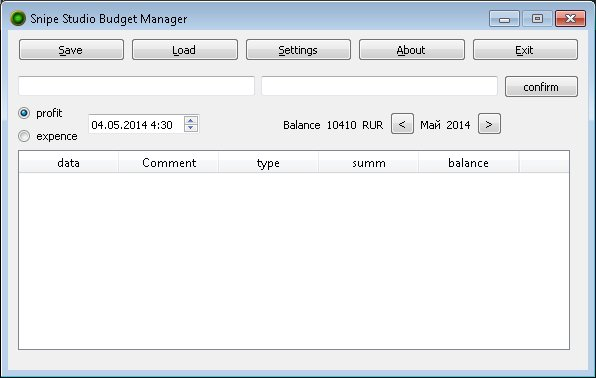
\includegraphics[width=0.7\linewidth]{pics/view1.jpeg}
	\caption{Окончательный вариант графического приложения Budget Manager}
	\label{fig:view1}
\end{figure}

Позже был изменен общий графический дизайн приложения 	и стал следующим:

\begin{figure}[H]
	\centering
	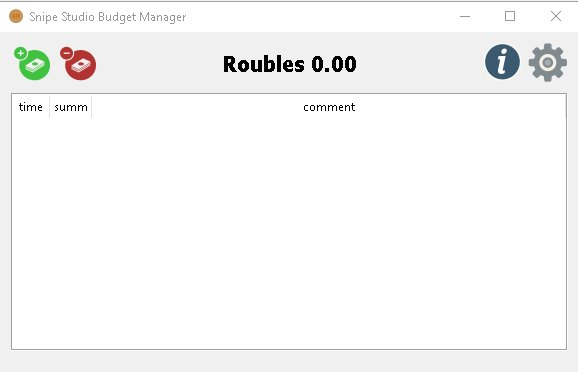
\includegraphics[width=0.7\linewidth]{pics/view2.jpeg}
	\caption{Второй вариант графического приложения Budget Manager}
	\label{fig:view2}
\end{figure}

Так же была собрана версия для Android

\begin{figure}[H]
	\centering
	
	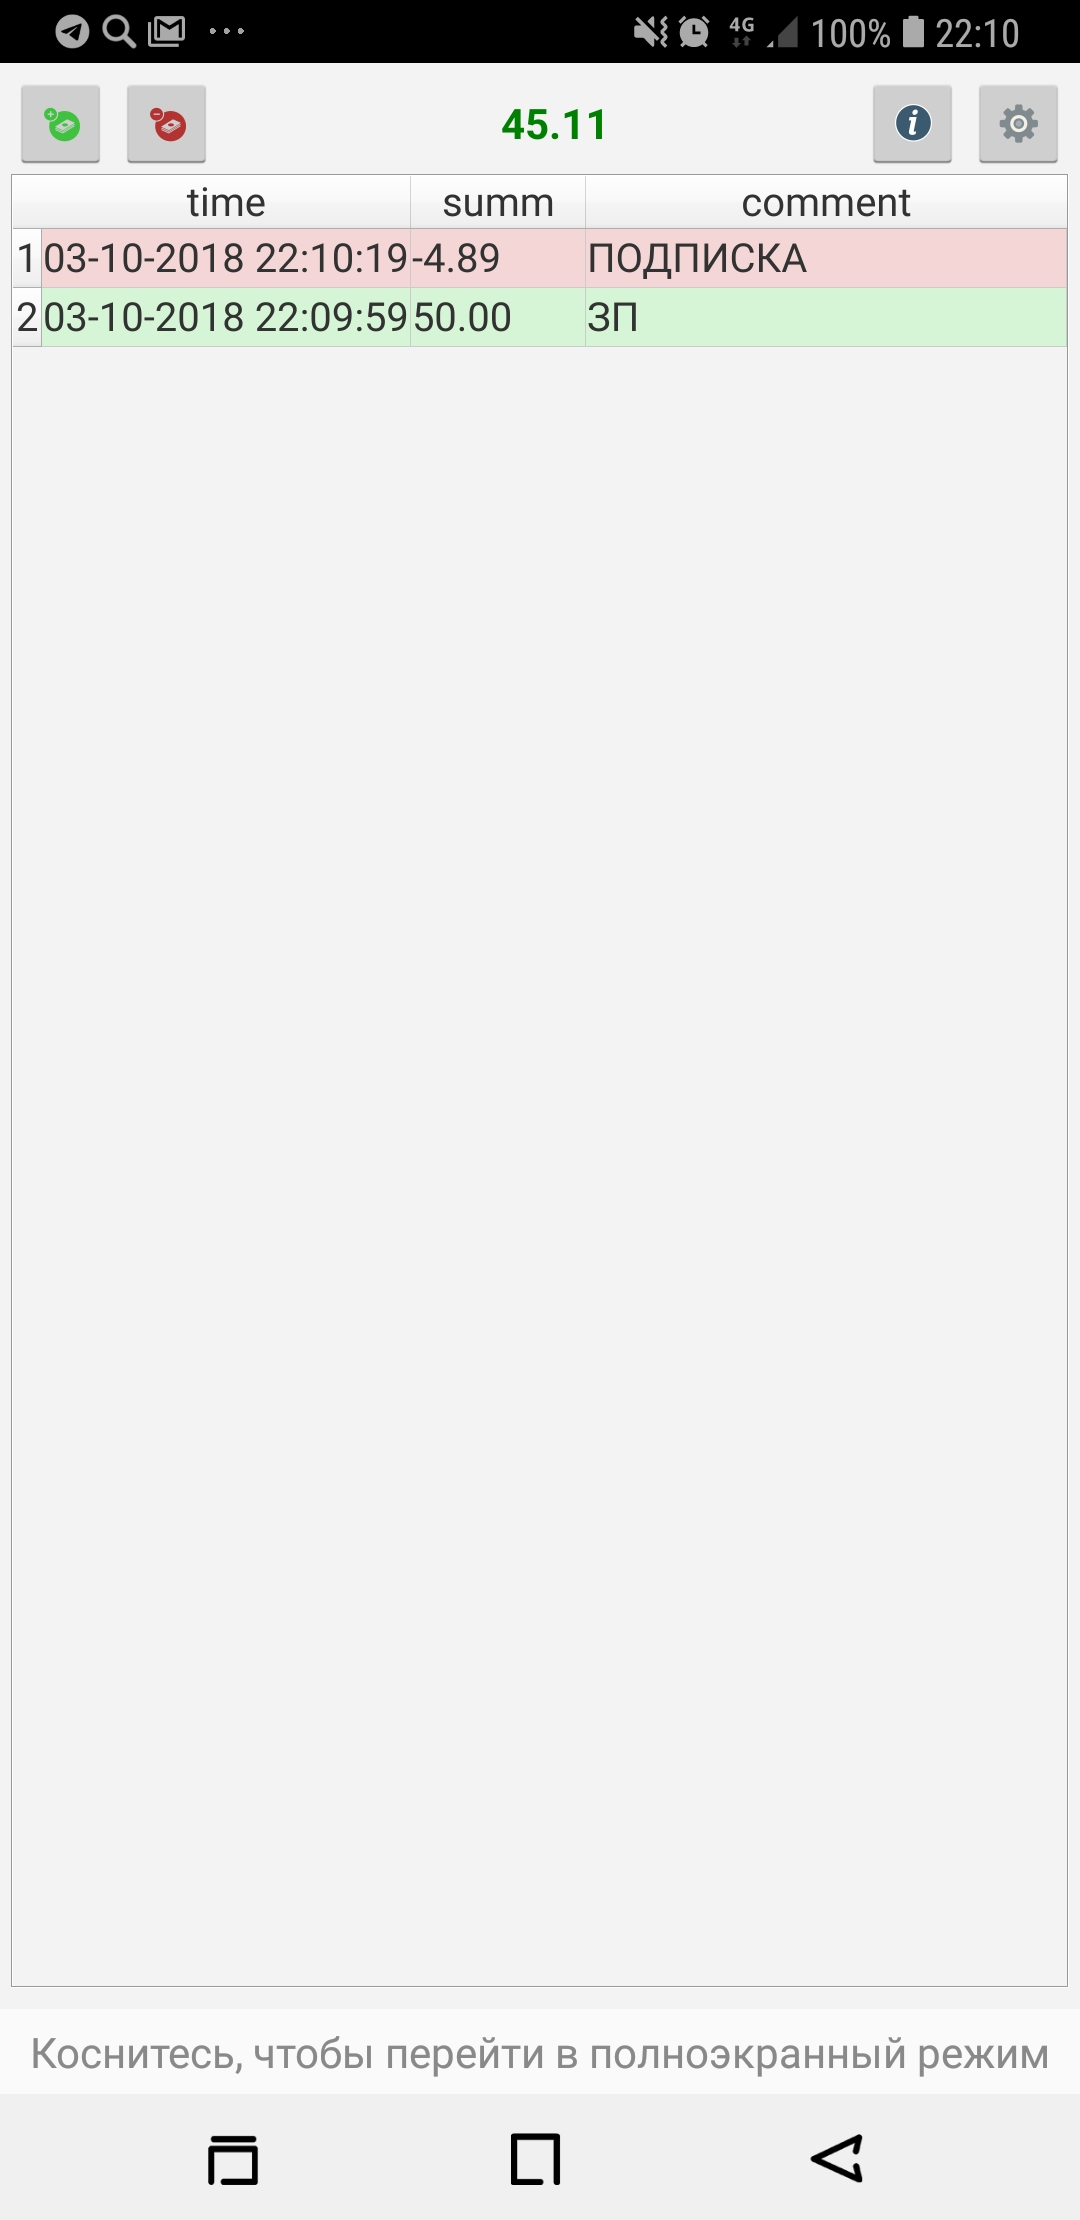
\includegraphics[height=0.7\linewidth]{pics/viewAndroid.jpeg}
	\caption{Версия для Android}
	\label{fig:viewAndroid}
\end{figure}